% paper-to-olympiad question booklet template (self-contained; compile twice with pdflatex)
\documentclass[11pt,a4paper]{article}
\usepackage[T1]{fontenc}
\usepackage[utf8]{inputenc}
\usepackage{fix-cm}
\usepackage[scaled=0.96]{helvet}
\renewcommand{\familydefault}{\sfdefault}
\usepackage{amsmath,amssymb,mathtools}
\usepackage{newtxmath}
\usepackage{bm,dsfont}
\usepackage[margin=20mm,top=35mm,bottom=20mm,headheight=57pt,headsep=10mm]{geometry}
\usepackage{microtype,booktabs,array,tabularx,enumitem,needspace}
\usepackage[most]{tcolorbox}
\usepackage{fancyhdr,lastpage,xcolor}
\usepackage{tikz}
\usetikzlibrary{arrows.meta,decorations.pathreplacing,decorations.pathmorphing,calc,positioning}
\usepackage{pgfplots}
\pgfplotsset{compat=1.18}
\usepackage[hidelinks,pdfencoding=auto,psdextra]{hyperref}
% ---------------- colours ----------------
\definecolor{ink}{HTML}{172A3A}
\definecolor{sourcegreen}{HTML}{1B6B4B}
\definecolor{sourcewash}{HTML}{F4FAF6}
\definecolor{openred}{HTML}{A42B32}
\definecolor{openwash}{HTML}{FFF6F6}
\definecolor{rulegray}{HTML}{5E6670}
\definecolor{figblue}{HTML}{2F5D8A}
\definecolor{figwash}{HTML}{F3F7FB}
\definecolor{colA}{HTML}{D9822B}
\definecolor{colB}{HTML}{3C78B4}
% ---------------- page ----------------
\setlength{\parindent}{0pt}
\setlength{\parskip}{5.4pt}
\setlength{\emergencystretch}{2em}
\raggedbottom
\newcommand{\booktitle}{TITLE OF THE PROBLEM}
\newcommand{\bookcode}{Q1}
\pagestyle{fancy}
\fancyhf{}
\fancyhead[L]{\begin{minipage}[b]{0.73\textwidth}\textbf{\large Theoretical Question Paper}\\[-1pt]{\small Olympiad-style guided problem \enspace|\enspace TOPIC}\\[-1pt]{\footnotesize English --- Revision 1}\end{minipage}}
\fancyhead[R]{\fontsize{29}{31}\selectfont\bfseries \bookcode-\thepage}
\renewcommand{\headrulewidth}{0.9pt}
\fancyfoot[L]{\footnotesize Not an official olympiad paper}
\fancyfoot[R]{\footnotesize \thepage/\pageref*{LastPage}}
% ---------------- notation helpers ----------------
\newcommand{\ket}[1]{\lvert #1\rangle}
\newcommand{\bra}[1]{\langle #1\rvert}
\newcommand{\Tr}{\operatorname{Tr}}
\newcommand{\dd}{\mathrm d}
\newcommand{\norm}[1]{\left\lVert #1\right\rVert}
\newcommand{\id}{\mathds 1}
% ---------------- structure ----------------
\newcommand{\parttitle}[3]{\par\vspace{2pt}{\large\bfseries\color{ink}Part #1. #2\hfill\normalsize(#3 points)}\par\vspace{4pt}}
\newcommand{\pagetitle}[1]{{\large\bfseries\color{ink}#1}\par\vspace{4pt}}
\newcommand{\smallheading}[1]{\par\Needspace{6\baselineskip}\medskip\textbf{#1}\par}
\newcommand{\nextpage}{\clearpage}
\newcommand{\flowtitle}[1]{\par\Needspace{14\baselineskip}\bigskip\pagetitle{#1}}
\newcommand{\origin}[1]{{\footnotesize\textbf{Source / scope:} #1}\par}
\newcommand{\hint}[1]{\par{\small\textbf{Hint.} #1}\par}
\newcommand{\handoff}[1]{\par\medskip{\small\textbf{Connection to the next step:} #1}\par}
\newcolumntype{Y}{>{\raggedright\arraybackslash}X}
% green = available with a named source; red = not established; blue = picture
\newtcolorbox{greenbox}[1]{enhanced,breakable,colback=sourcewash,colframe=sourcegreen,boxrule=0.9pt,arc=0pt,left=8pt,right=8pt,top=6pt,bottom=6pt,before skip=7pt,after skip=8pt,title={\strut AVAILABLE --- #1},colbacktitle=sourcewash,coltitle=sourcegreen,fonttitle=\bfseries\small,titlerule=0pt,fontupper=\small}
\newtcolorbox{redbox}[1]{enhanced,breakable,colback=openwash,colframe=openred,boxrule=0.9pt,arc=0pt,left=8pt,right=8pt,top=6pt,bottom=6pt,before skip=7pt,after skip=8pt,title={\strut NOT ESTABLISHED --- #1},colbacktitle=openwash,coltitle=openred,fonttitle=\bfseries\small,titlerule=0pt,fontupper=\small}
\tcbset{figstyle/.style={enhanced,breakable=false,colback=white,colframe=figblue,boxrule=0.8pt,arc=0pt,left=8pt,right=8pt,top=6pt,bottom=6pt,before skip=8pt,after skip=9pt,colbacktitle=figwash,coltitle=figblue,fonttitle=\bfseries\small,titlerule=0pt}}
\newcounter{figc}
\newenvironment{figpanel}[1]{\refstepcounter{figc}\begin{tcolorbox}[figstyle,title={\strut PICTURE \thefigc\ --- #1}]\centering}{\end{tcolorbox}}
\newcommand{\figtext}[1]{\par\smallskip{\raggedright\small #1\par}}
% scored boxes: \question{label}{points}{text}; \bridge and \extension take the same arguments
\newcommand{\question}[3]{\begin{tcolorbox}[enhanced,colback=white,colframe=rulegray,boxrule=0.5pt,arc=0pt,left=7pt,right=7pt,top=7pt,bottom=7pt,before skip=9pt,after skip=9pt]\begin{tabularx}{\linewidth}{@{}>{\bfseries}p{10mm}X>{\raggedleft\arraybackslash}p{13mm}@{}}#1&#3&\textbf{#2 pt}\end{tabularx}\end{tcolorbox}}
\newcommand{\bridge}[3]{\phantomsection\label{task:#1}\begin{tcolorbox}[enhanced,colback=white,colframe=ink,boxrule=0.7pt,arc=0pt,left=8pt,right=8pt,top=7pt,bottom=7pt,before skip=8pt,after skip=8pt]\textbf{#1}\hfill\textit{Modelling bridge}\quad\textbf{#2 pt}\par\smallskip #3\end{tcolorbox}}
\newcommand{\extension}[3]{\phantomsection\label{task:#1}\begin{tcolorbox}[enhanced,colback=white,colframe=rulegray,boxrule=0.5pt,arc=0pt,left=8pt,right=8pt,top=7pt,bottom=7pt,before skip=8pt,after skip=8pt]\textbf{#1}\hfill\textit{Supplement}\quad\textbf{#2 pt}\par\smallskip #3\end{tcolorbox}}
\tikzset{>={Stealth[length=2.2mm]},obj/.style={draw=ink,rounded corners=2pt,align=center,font=\small,inner sep=4pt,text width=31mm,fill=white},okarrow/.style={->,draw=ink,line width=0.9pt},openarrow/.style={->,draw=openred,dashed,line width=0.9pt}}
\pgfplotsset{mbaxis/.style={width=7.6cm,height=5.4cm,tick label style={font=\scriptsize},label style={font=\small},title style={font=\small},axis line style={rulegray},tick style={rulegray}}}
% ==== BEGIN GENERATED FIGURE DATA (your script) ====
\newcommand{\FigDataExample}{\addplot[colB,thick] coordinates {(0,0) (0.5,0.4) (1,0.6) (1.5,0.7) (2,1.0)};}
% ==== END GENERATED FIGURE DATA ====
\begin{document}

{\LARGE\bfseries\color{ink}\booktitle}\par
{\large Guided theory problem \hfill \textbf{10.0 points}}

\smallheading{How to use this booklet}
\begin{itemize}[leftmargin=6mm,itemsep=2pt,topsep=2pt]
\item Read the Background first. You do not need to read any paper.
\item Every question box shows its points. Every number, formula and assumption you need is printed here.
\item The Toolkit lists facts you may use without proof; the Glossary explains each technical word.
\item Blue PICTURE frames show what a question asks. They contain no answers.
\end{itemize}

\begin{greenbox}{How to read green frames}
A result you may use, with its source. Use it exactly as stated.
\end{greenbox}
\begin{redbox}{How to read red frames}
ADDED MODEL: a teaching model with an exact solution, not the real system. GIVEN BOUND: an assumption for an exercise. OPEN: still missing for the real system.
\end{redbox}

\smallheading{Points}
{\small\begin{tabularx}{\textwidth}{@{}p{9mm}Y r@{}}\toprule
Part&Questions&Points\\\midrule
A&A.1 (0.6), A.2 (0.9)&1.5\\
B&B.1 (1.0)&1.0\\\midrule
&&\textbf{2.5}\\\bottomrule
\end{tabularx}}

\smallheading{Notation (each symbol has one meaning)}
{\small\begin{tabularx}{\textwidth}{@{}p{30mm}Y@{}}\toprule
$H$&the Hamiltonian of the real system\\
$\mathcal K$&a generator in a chosen frame\\
$\id$&the identity\\\bottomrule
\end{tabularx}}

\nextpage
\pagetitle{Background. Everything you need to know}
\smallheading{1. The system}
Plain-language description of the system, with one picture.

\begin{figpanel}{The system}
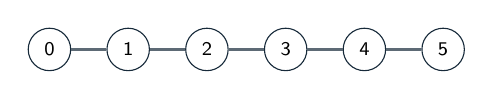
\begin{tikzpicture}[x=10mm,y=10mm]
\foreach \x in {0,...,5}{\node[circle,draw=ink,minimum size=5mm,font=\scriptsize] (n\x) at (\x,0) {\x};}
\foreach \x [evaluate=\x as \y using int(\x+1)] in {0,...,4}{\draw[ink!70,line width=1pt] (n\x)--(n\y);}
\end{tikzpicture}
\figtext{What is shown, in one sentence. \textbf{A.1 asks:} the question in plain words.}
\end{figpanel}

\smallheading{2. The mechanism}
\smallheading{3. The open question}

\nextpage
\pagetitle{Toolkit. Facts you may use without proof}
\begin{enumerate}[label=\textbf{T\arabic*.},leftmargin=9mm,itemsep=3pt]
\item \textbf{Change of frame.} If $i\partial_t\ket\psi=H\ket\psi$ and $\ket\xi=U^\dagger\ket\psi$, then $i\partial_t\ket\xi=(U^\dagger HU-iU^\dagger\dot U)\ket\xi$.
\end{enumerate}

\pagetitle{Glossary}
{\small\begin{tabularx}{\textwidth}{@{}>{\bfseries}p{34mm}Y@{}}\toprule
Term&Plain definition\\\bottomrule
\end{tabularx}}

\nextpage
\parttitle{A}{First part}{1.5}
\begin{greenbox}{PAPER [1] --- what the source states}
A short statement with its scope.
\end{greenbox}
\question{A.1}{0.6}{Find \dots. Explain \dots.}
\begin{redbox}{ADDED MODEL --- a teaching model}
Define the model and say what it is not.
\end{redbox}
\question{A.2}{0.9}{Find \dots. Does this establish \dots?}

\nextpage
\parttitle{B}{Second part}{1.0}
\begin{figpanel}{A computed picture}
\begin{tikzpicture}
\begin{axis}[mbaxis,xlabel={$t/T$},ylabel={quantity}]
\FigDataExample
\end{axis}
\end{tikzpicture}
\figtext{Computed from the model; state its scope. \textbf{B.1 asks:} \dots}
\end{figpanel}
\bridge{B.1}{1.0}{\textbf{(a)} Derive \dots.\par \textbf{(b)} Show \dots.}
\hint{Name the tool (e.g.\ T1), not the step.}

\nextpage
\pagetitle{Sources}
\begin{enumerate}[label={[\arabic*]},leftmargin=9mm]
\item Author, \emph{Title}, arXiv:xxxx.xxxxx.
\end{enumerate}
\vfill
\begin{center}\textbf{End of question booklet}\end{center}
\end{document}
